\documentclass[10pt]{article}
 
\usepackage[margin=1in]{geometry} 
\usepackage{amsmath,amsthm,amssymb, graphicx, multicol, array}
 
\newcommand{\N}{\mathbb{N}}
\newcommand{\Z}{\mathbb{Z}}
 

\begin{document}
 
\title{Homework 1}
\author{Juliette Franqueville\\
}
\maketitle
 
\section*{(5)}

\begin{figure}[!h]
    \centering
    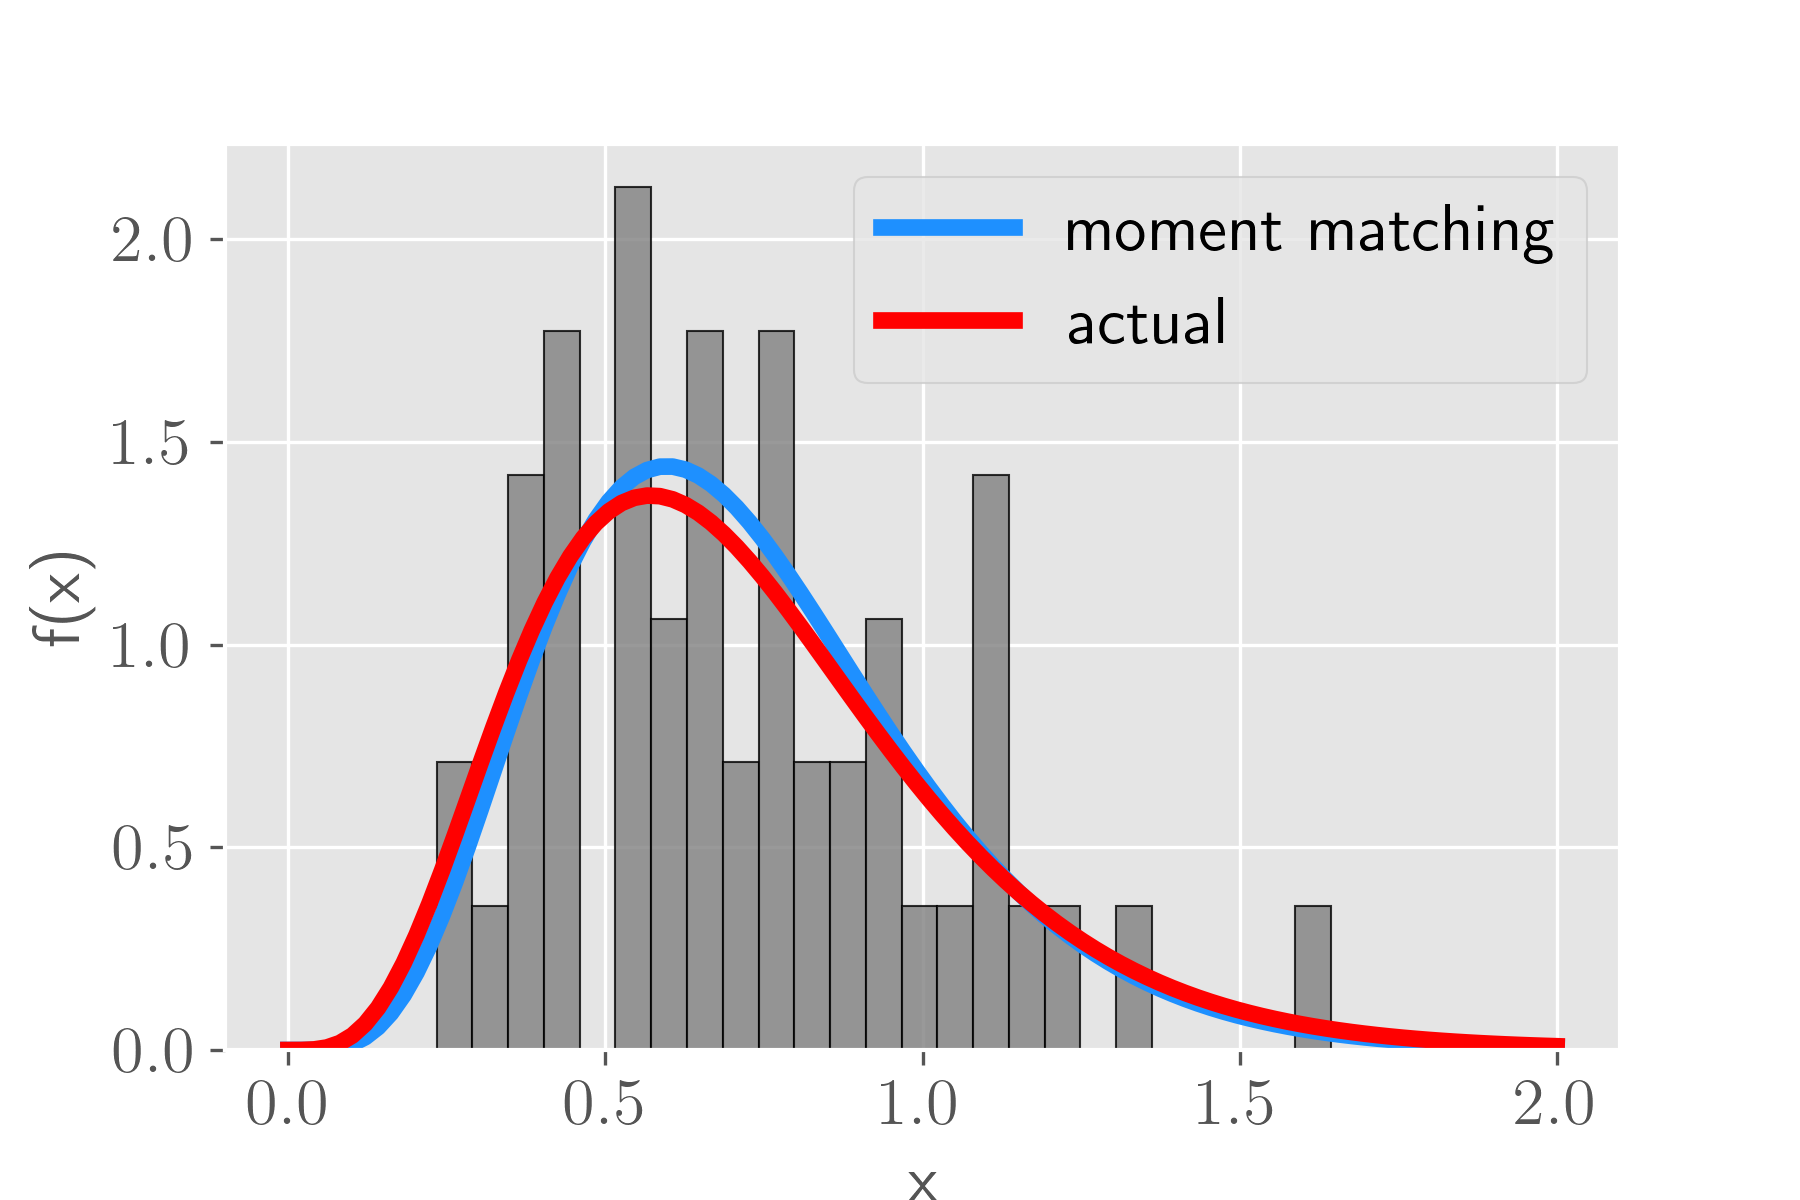
\includegraphics[scale=.7]{homework_1/first_hist.png}
    \caption{Caption}
    \label{fig:my_label}
\end{figure}

\begin{figure}[!h]
    \centering
    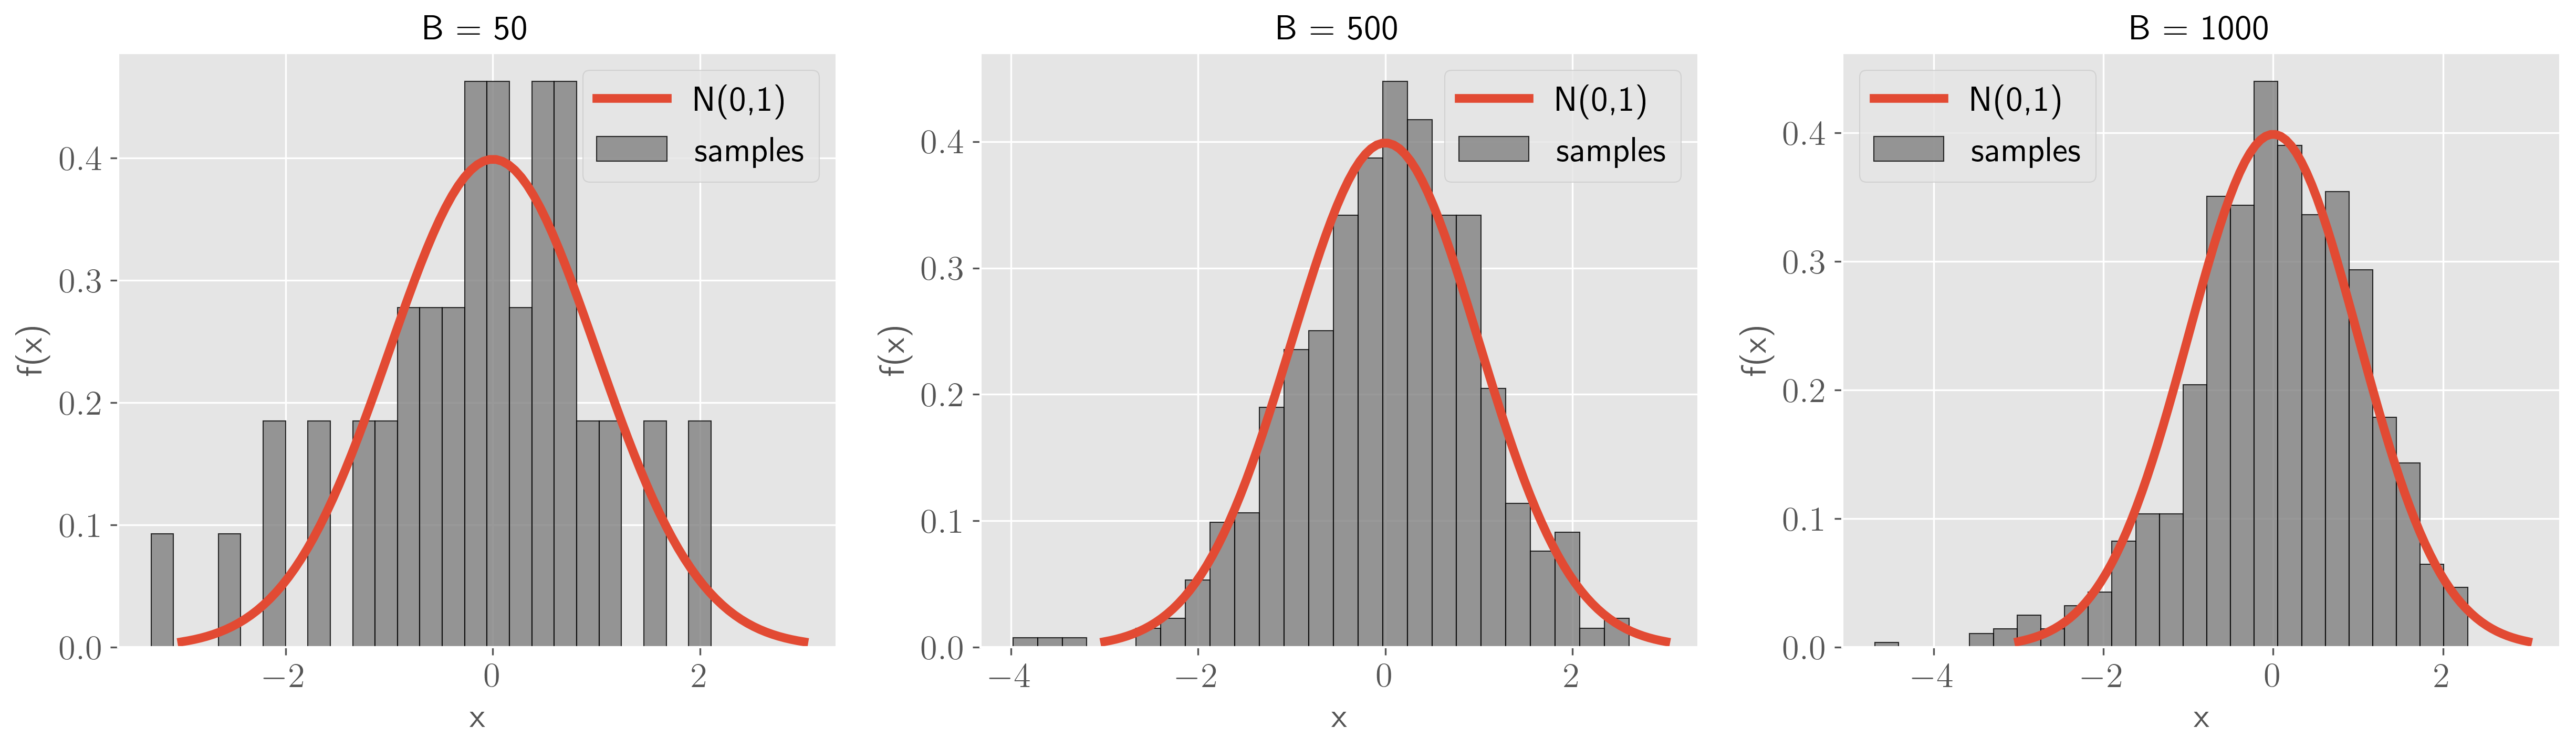
\includegraphics[scale=.35]{homework_1/second_hist.png}
    \caption{Caption}
    \label{fig:my_label}
\end{figure}


\begin{figure}[!h]
    \centering
    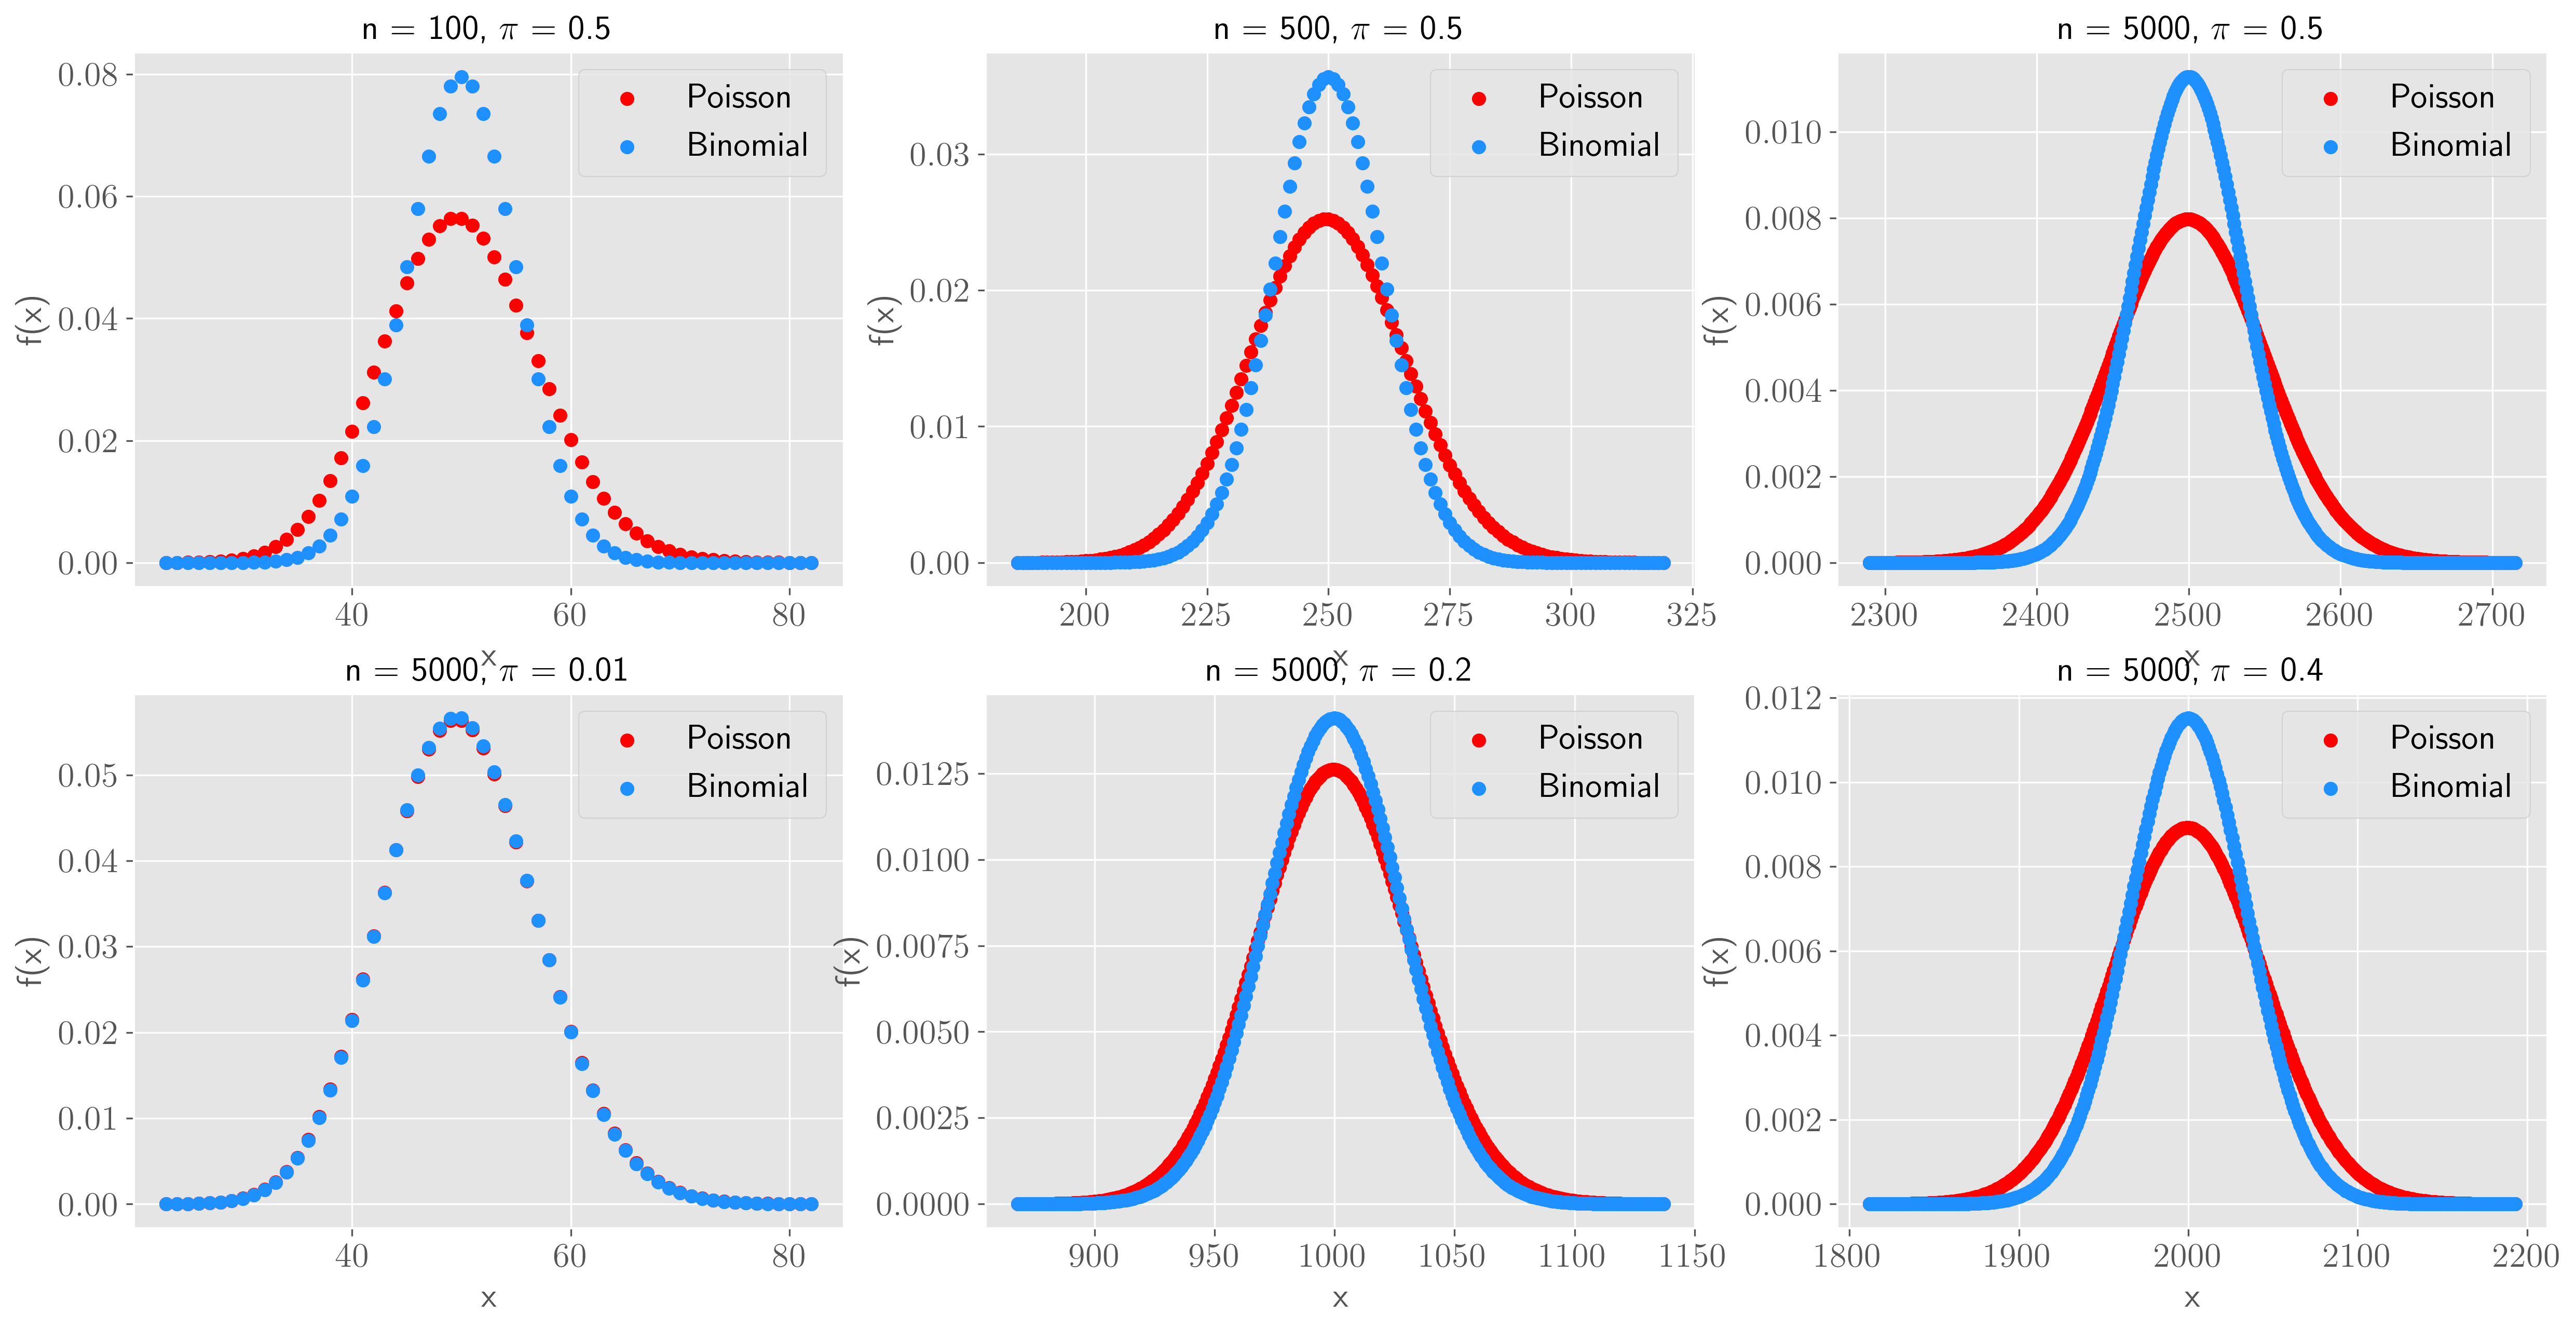
\includegraphics[scale=.35]{homework_1/third_hist.png}
    \caption{Caption}
    \label{fig:my_label}
\end{figure}



\end{document}